% The actual PGF smooth and constant plot paths form the edges, not the
% straight chords between their observations. The lower plateaus change
% height at x=1.75, 3.25 and 4.5; all geometry is in axis units of 1 cm.
\documentclass[border=2pt]{standalone}
\usepackage{pgfplots}
\usepgfplotslibrary{fillbetween}
\pgfplotsset{compat=1.18}
\begin{document}
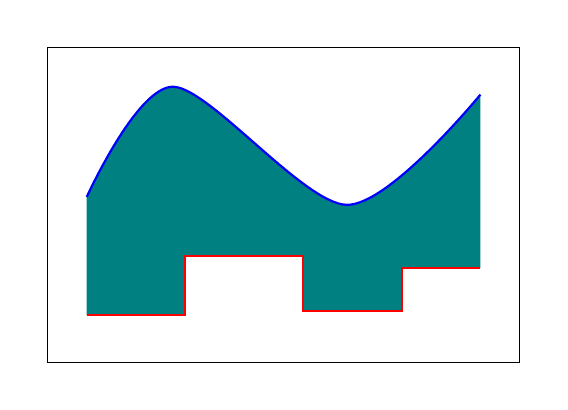
\begin{tikzpicture}
  \begin{axis}[at={(0,0)},anchor=south west,width=6cm,height=4cm,scale only axis,
    xmin=0,xmax=6,ymin=0,ymax=4,enlargelimits=false,axis lines=box,ticks=none]
    \addplot[blue,thick,mark=none,smooth,name path=upper]
      coordinates {(0.5,2.1) (1.6,3.5) (3.8,2.0) (5.5,3.4)};
    \addplot[red,thick,mark=none,const plot,name path=lower]
      coordinates {(0.5,0.6) (1.75,1.35) (3.25,0.65) (4.5,1.2) (5.5,1.2)};
    \addplot[draw=none,fill=teal] fill between[of=upper and lower];
  \end{axis}
  \path[use as bounding box] (-0.25,-0.25) rectangle (6.25,4.25);
\end{tikzpicture}
\end{document}
